%Packages
\usepackage{amsmath,amssymb,amsfonts,graphicx,tikz-cd,mathtools,amsthm,amsxtra,geometry,parskip}
\usepackage{caption}
\usepackage{subcaption}

%Setup document
\geometry{margin = 1in}
\newtheoremstyle{break}% name
  {}%         Space above, empty = `usual value'
  {2em}%         Space below
  {\normalfont}% Body font
  {}%         Indent amount (empty = no indent, \parindent = para indent)
  {\bfseries}% Thm head font
  {.}%        Punctuation after thm head
  {\newline}% Space after thm head: \newline = linebreak
  {}%         Thm head spec

%Macros
\newcommand{\HOM}{\text{Hom}}
\newcommand{\CC}{\mathbb{C}}
\newcommand{\RR}{\mathbb{R}}
\newcommand{\QQ}{\mathbb{Q}}
\newcommand{\ZZ}{\mathbb{Z}}
\newcommand{\NN}{\mathbb{N}}
\theoremstyle{break}
\newtheorem{problem}{Problem}
\theoremstyle{definition}
\newtheorem{definition}{Definition}
\newtheorem{example}{Example}
\newtheorem{remark}{Remark}
\newtheorem{solution}{Solution}

% Make TOC clickable
\usepackage{hyperref}
\hypersetup{
    colorlinks,
    citecolor=black,
    filecolor=black,
    linkcolor=black,
    urlcolor=black
}

% Highlight quote
\usepackage{xcolor}
\usepackage{environ}
\definecolor{block-gray}{gray}{0.85}
\NewEnviron{myblock}
{\colorbox{block-gray}{%
\parbox{\dimexpr\linewidth-2\fboxsep\relax}{%
\small\addtolength{\leftskip}{10mm}
\addtolength{\rightskip}{10mm}
\BODY}}
}
\renewcommand{\quote}{\myblock}
\renewcommand{\endquote}{\endmyblock}

% Macros
\renewcommand{\vector}[1]{\mathbf{#1}}
\newcommand{\NN}[0]{{\mathbb{N}}}
\newcommand{\RR}[0]{{\mathbb{R}}}
\newcommand{\ZZ}[0]{{\mathbb{Z}}}
\newcommand{\CC}[0]{{\mathbb{C}}}
\newcommand{\QQ}[0]{{\mathbb{Q}}}
\newcommand{\RP}[0]{{\mathbb{RP}}}
\newcommand{\CP}[0]{{\mathbb{CP}}}
\newcommand{\HP}[0]{{\mathbb{HP}}}
\newcommand{\OP}[0]{{\mathbb{OP}}}
\newcommand{\FF}[0]{{\mathbb{F}}}
\newcommand{\GF}[0]{{\mathbb{GF}}}
\newcommand{\PP}[0]{{\mathbb{P}}}
\newcommand{\Af}[0]{{\mathbb{A}}}
\newcommand{\MM}[0]{{\mathbb{M}}}
\newcommand{\TT}[0]{{\mathbb{T}}}
\newcommand{\Sp}[0]{{\mathbb{S}}}
\newcommand{\KK}[0]{{\mathbb{K}}}
\newcommand{\Gr}[0]{{\text{Gr}}}
\newcommand{\GL}[0]{{\text{GL}}}
\newcommand{\liegl}[0]{{\mathfrak{gl}}}
\newcommand{\lieg}[0]{{\mathfrak{g}}}
\newcommand{\lieh}[0]{{\mathfrak{h}}}
\newcommand{\SL}[0]{{\text{SL}}}
\newcommand{\liesl}[0]{{\mathfrak{sl}}}
\newcommand{\SP}[0]{{\text{SP}}}
\newcommand{\liesp}[0]{{\mathfrak{sp}}}
\newcommand{\SO}[0]{{\text{SO}}}
\newcommand{\lieso}[0]{{\mathfrak{so}}}
\newcommand{\OO}[0]{{\mathcal{O}}}
\newcommand{\mm}[0]{{\mathfrak{m}}}
\newcommand{\pr}[0]{{\mathfrak{p}}}
\newcommand{\mltext}[1]{\left\{\begin{array}{c}#1\end{array}\right\}}
\newcommand{\dual}[0]{^\vee}
\newcommand{\Tr}[0]{\mathrm{Tr}}
\newcommand{\tr}[0]{\mathrm{Tr}}
\def\endo{\operatorname{End}}
\def\Endo{\operatorname{End}}
\def\Ind{\operatorname{End}}
\def\ind{\operatorname{End}}
\newcommand{\divides}[0]{{~\Bigm| ~}}
\newcommand{\notdivides}[0]{{~\not\Bigm| ~}}
\newcommand{\sym}[0]{\mathrm{Sym}}
\newcommand{\aut}[0]{\mathrm{Aut}}
\newcommand{\grad}[0]{\mathrm{grad}}
\newcommand{\sign}[0]{\mathrm{sign}}
\newcommand{\spec}[0]{{\mathrm{Spec}}}
\newcommand{\spanof}[0]{{\mathrm{span}}}
%\newcommand{\suchthat}[0]{{~\backepsilon ~}}
\newcommand{\suchthat}[0]{{~\mathrel{\Big|}~}}
\newcommand{\uniformlyconverges}[0]{\rightrightarrows}
\newcommand{\mapsvia}[1]{\xrightarrow{#1}}
\newcommand{\converges}[1]{\overset{#1}}
\newcommand{\generators}[1]{\left\langle{#1}\right\rangle}
\newcommand{\theset}[1]{\left\{{#1}\right\}}
\newcommand{\too}[1]{{\xrightarrow{#1}}}
\newcommand{\correspond}[1]{\theset{\substack{#1}}}
\newcommand{\restrictionof}[2]{{\left.{#1}\right|_{#2}}}
\newcommand{\inner}[2]{{\left\langle {#1},~{#2} \right\rangle}}
\newcommand{\indicator}[1]{{\unicode{x1D7D9}\left[#1\right]}}
\newcommand{\equalsbecause}[1]{{\stackrel{\mbox{$\tiny{\text{ #1 }}$}}{=}}}
\newcommand{\conjugate}[1]{{\overline{{#1}}}}
\newcommand{\strike}[1]{{\enclose{horizontalstrike}{#1}}}
\newcommand{\realpart}[1]{{\mathcal{Re}({#1})}}
\newcommand{\imaginarypart}[1]{{\mathcal{Im}({#1})}}
\newcommand{\dd}[2]{{\frac{\partial #1}{\partial #2}}}
\newcommand{\rotate}[2]{{\style{display: inline-block; transform: rotate(#1deg)}{#2}}}
\newcommand{\stirling}[2]{\genfrac\{\}{0pt}{}{#1}{#2}}
\newcommand{\thevector}[1]{{\left[ {#1} \right]}}
%\newcommand{\abs}[2]{{\left\lvert {#2} \right\rvert_{\text{#1}}}}
\newcommand{\norm}[1]{{\left\lVert {#1} \right\rVert}}
\newcommand{\abs}[1]{{\left\lvert {#1} \right\rvert}}
\newcommand{\intersect}[0]{\bigcap}
\newcommand{\union}[0]{\bigcup}
\newcommand{\coker}[0]{\operatorname{coker}}
\newcommand{\rank}[0]{\operatorname{rank}}
\newcommand{\tensor}[0]{\otimes}
\newcommand{\semidirect}[0]{\rtimes}
\newcommand{\pt}[0]{\{\text{pt}\}}
\newcommand{\bd}[0]{{\del}}
\newcommand{\wait}[0]{{\,\cdot\,}}
\newcommand{\selfmap}[0]{{\circlearrowleft}}
\newcommand{\tor}[0]{\text{Tor}}
\newcommand{\Tor}[0]{\text{Tor}}
\newcommand{\ext}[0]{\text{Ext}}
\newcommand{\actson}[0]{\curvearrowright}
\newcommand{\actsonl}[0]{\curvearrowleft}
\newcommand{\disjoint}[0]{{\coprod}}
\newcommand{\dash}[0]{{\hbox{-}}}
\newcommand{\bigast}[0]{{\mathop{\Large \ast}}}
\newcommand{\from}[0]{\leftarrow}
\newcommand{\covers}[0]{\twoheadrightarrow}
\newcommand{\Zp}[0]{\mathbb{Z}_{(p)}}
\newcommand{\Qp}[0]{\mathbb{Q}_{(p)}}
\newcommand{\ZpZ}[0]{\mathbb{Z}/p\mathbb{Z}}
\newcommand{\ZnZ}[0]{\mathbb{Z}/n\mathbb{Z}}
\newcommand{\Sm}[0]{{\text{Sm}_k}}
\newcommand{\GG}[0]{{\mathbb{G}}}
\newcommand{\bung}[0]{\text{Bun}_G}
\newcommand{\Aut}[0]{{\text{Aut}}}
\newcommand{\del}[0]{{\partial}}
\newcommand{\im}[0]{{\text{im}~}}
\newcommand{\homotopic}[0]{\simeq}
\newcommand{\into}[0]{\to}
\newcommand{\cross}[0]{\times}
\newcommand{\definedas}[0]{\coloneqq}
\newcommand{\surjects}[0]{\twoheadrightarrow}
\newcommand{\onto}[0]{\twoheadrightarrow}
\newcommand{\injects}[0]{\hookrightarrow}
\newcommand{\id}[0]{\text{id}}
\newcommand{\inv}[0]{^{-1}}
\newcommand{\normal}[0]{{~\trianglelefteq~}}
\newcommand{\trianglerightneq}{\mathrel{\ooalign{\raisebox{-0.5ex}{\reflectbox{\rotatebox{90}{$\nshortmid$}}}\cr$\triangleright$\cr}\mkern-3mu}}
\newcommand{\normalneq}{\mathrel{\reflectbox{$\trianglerightneq$}}}
\newcommand{\units}[0]{^{\times}}
\newcommand{\annd}[0]{{\text{ and }}}
\newcommand{\orr}[0]{{\text{ or }}}
\newcommand{\arcsec}[0]{\mathrm{arcsec}}
\newcommand{\Gal}[0]{\mathrm{Gal}}
\newcommand{\gal}[0]{\mathrm{Gal}}
\newcommand{\ann}[0]{\mathrm{Ann}}
\newcommand{\lcm}[0]{\mathrm{lcm}}
\newcommand{\multinomial}[1]{\left(\!\!{#1}\!\!\right)}
\newcommand{\stirlingfirst}[2]{\genfrac{[}{]}{0pt}{}{#1}{#2}}
\newcommand{\floor}[1]{{\left\lfloor #1 \right\rfloor}}
\newcommand{\ad}[0]{\mathrm{ad}~}
\newcommand{\ch}[0]{\mathrm{char}~}
\renewcommand{\mid}[0]{\mathrel{\Big|}}
%\newcommand{\vector}[1]{{\mathbf{ {#1} }}}
%\newcommand{\hom}[0]{\text{Hom}}
%\newcommand{\qed}[0]{{\tag*{$\blacksquare$}}}
\renewcommand{\qed}[0]{\hfill\blacksquare}
%\renewcommand{\qed}[0]{\eqno\qed}
%\newcommand{\char}[0]{\text{char}}

\let\Begin\begin
\let\End\end
\newcommand\wrapenv[1]{#1}

\makeatletter
\def\ScaleWidthIfNeeded{%
 \ifdim\Gin@nat@width>\linewidth
    \linewidth
  \else
    \Gin@nat@width
  \fi
}
\def\ScaleHeightIfNeeded{%
  \ifdim\Gin@nat@height>0.9\textheight
    0.9\textheight
  \else
    \Gin@nat@width
  \fi
}
\makeatother

\setkeys{Gin}{width=\ScaleWidthIfNeeded,height=\ScaleHeightIfNeeded,keepaspectratio}%

\title{
\textbf{
    Title
  }
  }
\author{D. Zack Garza}
\date{\today}

\begin{document}

\maketitle
% \todo{Insert title and subtitle.}
\tableofcontents


\hypertarget{thursday-january-9th}{%
\section{Thursday January 9th}\label{thursday-january-9th}}

\textbf{Recall:} For \(M^n\) a closed smooth manifold, consider a smooth
map \(f: M^n \to \RR\).

\textbf{Definition:} A critical point \(p\) of \(f\) is
\emph{non-degenerate} iff
\(\det( H\definedas \frac{\del^i f}{\del x_i \del x_j}(p)) \neq 0\) in
some coordinate system \(U\).

\textbf{Lemma (The Morse Lemma)}: For any non-degenerate critical point
\(p\) there exists a coordinate system around \(p\) such that

\begin{align*}
f(x_1, \cdots, x_n) = f(p) - x_1^2 - x_2^2 - \cdots - x_\lambda^2 + x_{\lambda+1}^2 + \cdots + x_n^2
.\end{align*}

\(\lambda\) is called the \emph{index of \(f\) at \(p\)}.

\textbf{Lemma:} \(\lambda\) is equal to the number of \emph{negative}
eigenvalues of \(H(p)\).

\emph{Proof:} A change of coordinates sends \(H(p) \to A^t H(p) A\),
which (exercise) has the same number of positive and negative values.

\begin{quote}
Exercise: show this assuming that \(A\) is invertible and not
necessarily orthogonal. Use the fact that \(A^t H A\) is diagonalizable.
\end{quote}

This means that \(f\) can be written as the quadratic form

\begin{align*}
\left[\begin{array}{ccccc}
-2  & 0  & 0       & 0    & 0 \\
0   & -2 & 0       & 0    & 0 \\
0   & 0  & \ddots  &  0   & 0 \\
0   & 0  & 0       &  2   & 0 \\
0   & 0  & 0       &  0   & 2
\end{array}\right]
.\end{align*}

\emph{Proof of Morse Lemma:}

Suppose that we have a coordinate chart \(U\) around \(p\) such that
\(p\mapsto 0\in U\) and \(f(p) = 0\).

\textbf{Step 1 -- Claim:} There exists a coordinate system around \(p\)
such that

\begin{align*}
f(x) = \sum_{i,j=1}^n x_i x_j h_{ij}(x)
,\end{align*}

where \(h_{ij}(x) = h_{ji}(x)\).

\emph{Proof:} Pick a convex neighborhood \(V\) of \(0\in \RR^n\).

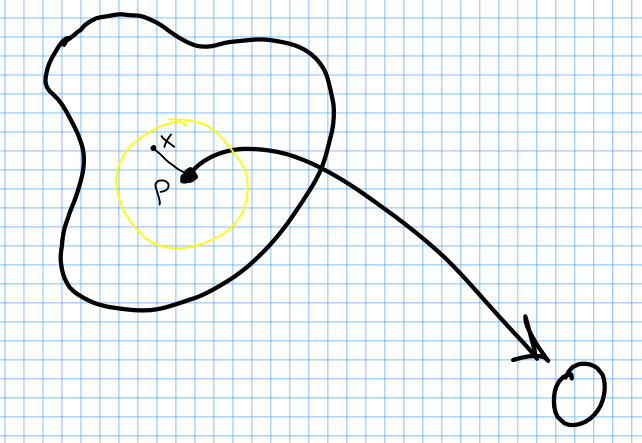
\includegraphics{figures/2020-01-09-11:38.png}\\

Restrict \(f\) to a path between \(x\) and \(0\), and by the FTC compute

\begin{align*}
I = \int_0^1 \frac{df(tx_1, tx_2, \cdots, tx_n) }{dt}  ~dt = f(x_1, \cdots, x_n) - f(0) = f(x_1, \cdots, x_n)
.\end{align*}

since \(f(0) = 0\).

We can compute this in a second way, \begin{align*}
I = \int_0^1 \dd{f}{x_1} x_1 + \dd{f}{x_2} x_2 + \cdots \dd{f}{x_n} x_n ~dt 
\implies \sum_{i=1}^n x_i \int_0^1  \dd{f}{x_i} ~dt = f(x)
.\end{align*}

We thus have \(f(x) = \sum_{i=1}^n x_i g_i(x)\) where
\(\dd{f}{x_i}(0) = 0\), and
\(\dd{f}{x_i} = x_1 \dd{g_1}{x_i} + \cdots + g_i + x_i \dd{g_i}{x_i} + \cdots + x_n \dd{g_n}{x_i}\).

When we plug \(x = 0\) into this expression, the only term that doesn't
vanish is \(g_i\), and thus \(\dd{f}{x_i}(0) = g_i(0)\) and
\(g_i(0) = 0\).

Applying the same result to \(g_i\), we obtain
\(g_i(x) = \sum_{j=1}^n x_j h_{ij}(x)\), and thus
\(f(x) = \sum_{i, j =1}^n x_i x_j h_{ij}(x)\).

We still need to show \(h\) is symmetric. For every pair \(i, j\), there
is a term of the form \(x_i x_j h_{ij} + x_j x_i h_{ji}\). So let
\(H_{ij}(x) = \frac{h_{ij}(x) + h_{ji}(x)}{2}\) (i.e.~symmetrize/average
\(h\)), then \(f(x) = \sum_{i, j = 1}^n x_i x_j H_{ij}(x)\) and this
shows claim 1.

\(\qed\)

\textbf{Step 2 -- Induction:} Assume that in some coordinate system
\(U_0\),

\begin{align*}
f(y_1, \cdots, y_n) = \pm y_1^2 \pm y_2^2 \pm \cdots \pm y_{r-1}^2 + \sum_{i, j \geq r} y_i y_j H_{ij}(y_1, \cdots, y_n)
.\end{align*}

Note that \(H_{rr}(0)\) is given by the top-left block of \(H_{ij}(0)\),
which is thus looks like

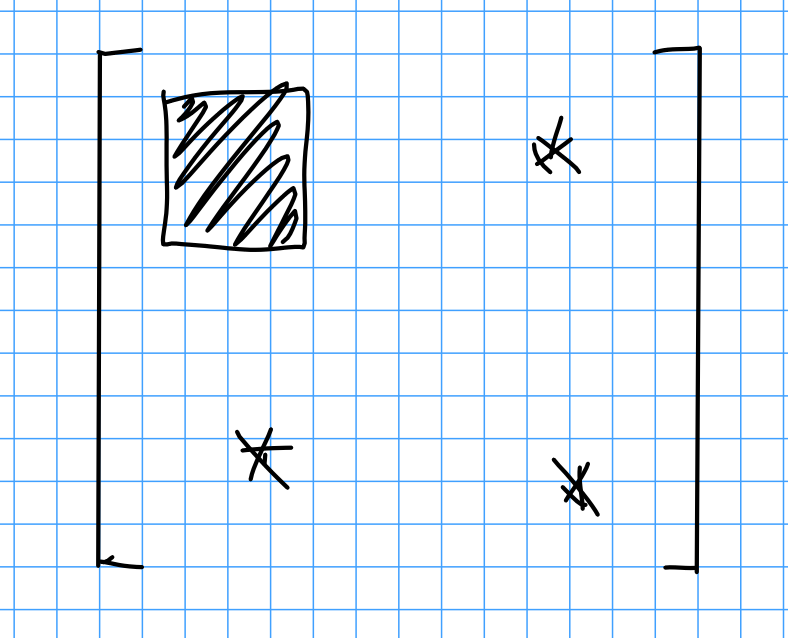
\includegraphics{figures/2020-01-09-11:41.png}\\

Note that this block is symmetric.

Claim 1: There exists a linear change of coordinates such that
\(H_{rr}(0) \neq 0\).

We can use the fact that
\(\frac{\del^2 f}{\del x_i \del x_j} (0) = H_{ij}(0) + H_{ji}(0) = 2 H_{ij}(0)\),
and thus
\(H_{ij}(0) = \frac{1}{2} \left( \frac{\del f}{\del x_i \del x_j} \right)\).

Since \(H(0)\) is non-singular, we can find \(A\) such that
\(A^t H(0) A\) has nonzero \(rr\) entry, namely by letting the first
column of \(A\) be an eigenvector of \(H(0)\), then
\(A = [\vector v, \cdots]\) and thus
\(H(0)A = [\lambda \vector v, \cdots]\) and
\(A^t[\lambda \vector v] = [\lambda \norm{\vector v}^2, \cdots ]\).

So

\begin{align*}
\sum_{i,j\geq r} y_i y_j H_{ij}(y_1, \cdots, y_n) 
&= y_r^2 H_{rr}(y_1, \cdots, y_n) + \sum_{i > r} 2y_i y_r H_{ir}(y_1, \cdots, y_n) \\
&= H_{rr}(y_1, \cdots, y_n) \left( 
y_r^2 + \sum_{i > r} 2y_i y_r H_{ir}(y_1, \cdots, y_n)/H_{rr}(y_1, \cdots, y_n)
\right) \\
&= H_{rr}(y_1, \cdots, y_n) \left(
\left( y_r + \sum_{i > r}^n y_i H_{ir}(y_1, \cdots, y_n) / )_{rr}(y_1, \cdots, y_n) \right)^2
\sum_{i > r}^n y_i^2 \left( H_{ir}Y/H_{rr}(Y) \right)^2
\sum_{i, j > r}^n H_{ir}(Y)H_{jr}(Y)/H_{rr}(Y)
\right)^2 \quad\text{by completing the square}
.\end{align*}

\begin{quote}
Note that \(H_{rr}(0) \neq 0\) implies that \(H_{rr} \neq 0\) in a
neighborhood of zero as well.
\end{quote}

Now define a change of coordinates \(\phi: U \to \RR^n\) by
\begin{align*}
z_i = \begin{cases}
y_i & i\neq r \\
\sqrt{ H_{rr}(y_1, \cdots, y_n) } \left( y_r + \sum_{i> r} y_i H_{ir}(Y)/H_{rr}(Y) \right) & i=r
\end{cases}
.\end{align*}

This means that
\(f(z) = \pm z_1^2 \pm \cdots \pm z_{r-1}^2 \pm z_r^2 + \sum_{i, j \geq r+1^n z_i z_j \tilde{H}(z_1, \cdots, z_n) }\).

\begin{quote}
Exercise: show that \(d_0\phi\) is invertible, and by the inverse
function theorem, conclude that there is a neighborhood
\(U_2 \subset U_1\) of 0 on which \(\phi\) is still invertible.
\end{quote}

\(\qed\)

\textbf{Corollary:} The nondegenerate critical points of a Morse
function \(f\) are isolated.

\emph{Proof:} In some neighborhood around \(p\), we have
\(f(x) = f(p) - x_1^2 - \cdots - x_\lambda^2 + x_{\lambda + 1}^2 + \cdots + x_n^2\),
Thus \(\dd{f}{x_i} = 2x_i\), and so \(\dd{f}{x_i} = 0\) iff
\(x_1 = x_2 = \cdots = x_n = 0\).

\textbf{Corollary:} On a closed (compact) manifold \(M\), a Morse
function has only finitely many critical points.

We will need these facts to discuss the \(h\dash\)cobordism theorem. For
a closed smooth manifold, \(\del M = \emptyset\), so \(M\) will define a
cobordism \(\emptyset \to \emptyset\).

\textbf{Definition:} Let \(W\) be a cobordism from \(M_0 \to M_1\). A
\emph{Morse function} is a smooth map \(f: W\to [a, b]\) such that

\begin{enumerate}
\def\labelenumi{\arabic{enumi}.}
\tightlist
\item
  \(f\inv(a) = M_0\) and \(f\inv(b) = M_1\),
\item
  All critical points of \(f\) are non-degenerate and contained in
  \(\mathrm{int}(W) \definedas W\setminus \del W\).
\end{enumerate}

\begin{quote}
So \(f\) is equal to the endpoints only on the boundary.
\end{quote}

\begin{quote}
Next time: existence of Morse functions. This is a fairly restrictive
notion, but they are dense in the \(C^2\) topology on (?).
\end{quote}

%\listoftodos

\bibliography{/home/zack/Notes/library.bib}

\end{document}
